%! Author = Simone
%! Date = 17/03/2023

% Preamble
\documentclass[11pt, a4paper]{article}

%------------------------------------------------------------------------------
%	REQUIRED PACKAGES AND  CONFIGURATIONS
%------------------------------------------------------------------------------
% PACKAGES FOR TITLES
\usepackage{titlesec}
\usepackage{color}

% PACKAGES FOR LANGUAGE AND FONT
\usepackage[utf8]{inputenc}
\usepackage[english]{babel}
\usepackage[T1]{fontenc} % Font encoding

% PACKAGES FOR IMAGES
\usepackage{graphicx}
\graphicspath{{Images/}}
\usepackage{eso-pic} % For the background picture on the title page
\usepackage{subfig} % Numbered and caption subfigures using \subfloat
\usepackage{caption} % Coloured captions
\usepackage{transparent}

% STANDARD MATH PACKAGES
\usepackage{amsmath}
\usepackage{bm}
\usepackage[overload]{empheq}  % For braced-style systems of equations

% PACKAGES FOR TABLES
\usepackage{tabularx}
\usepackage{longtable} % tables that can span several pages
\usepackage{colortbl}

% PACKAGES FOR ALGORITHMS (PSEUDO-CODE)
\usepackage{algorithm}
\usepackage{algorithmic}

% PACKAGES FOR REFERENCES & BIBLIOGRAPHY
\usepackage[colorlinks=true,linkcolor=black,anchorcolor=black,citecolor=black,filecolor=black,menucolor=black,runcolor=black,urlcolor=black]{hyperref} % Adds clickable links at references
\usepackage{cleveref}
\usepackage[square, numbers, sortcompress]{natbib} % Square brackets, citing references with numbers, citations sorted by appearance in the text and compressed
\bibliographystyle{plain} % You may use a different style adapted to your field

% PACKAGES FOR THE APPENDIX
\usepackage{appendix}

% PACKAGES FOR ITEMIZE & ENUMERATES
\usepackage{enumitem}

% OTHER PACKAGES
\usepackage{amsthm,thmtools,xcolor} % Coloured "Theorem"
\usepackage{comment} % Comment part of code
\usepackage{fancyhdr} % Fancy headers and footers
\usepackage{lipsum} % Insert dummy text
\usepackage{tcolorbox} % Create coloured boxes (e.g. the one for the key-words)

%   PERSONAL PACKAGES
\usepackage{tikz}
\usetikzlibrary{automata, positioning, arrows}



%   COMMANDS
%\newcommand{\bea}{\begin{eqnarray}} % Shortcut for equation arrays
%\newcommand{\eea}{\end{eqnarray}}
%\newcommand{\e}[1]{\times 10^{#1}}  % Powers of 10 notation
%\newcommand{\mathbbm}[1]{\text{\usefont{U}{bbm}{m}{n}#1}} % From mathbbm.sty
%\newcommand{\pdev}[2]{\frac{\partial#1}{\partial#2}}

% Do not change Configuration_files/config.tex file unless you really know what you are doing.
% This file ends the configuration procedures (e.g. customizing commands, definition of new commands)
% Configuration package
\usepackage[bottom=2.0cm,top=2.0cm,left=2.0cm,right=2.0cm]{geometry}
\raggedbottom

% Create color bluePoli (-> manuale grafica coordinata:  https://www.polimi.it/fileadmin/user_upload/il_Politecnico/grafica-coordinata/2015_05_11_46xy_manuale_grafica_coordinata.pdf)
\definecolor{bluePoli}{cmyk}{0.4,0.1,0,0.4}

% Custom theorem environments
\declaretheoremstyle[
    headfont=\color{bluePoli}\normalfont\bfseries,
    bodyfont=\color{black}\normalfont\itshape,
]{colored}

\captionsetup[figure]{labelfont={color=bluePoli}} % Set colour of the captions
\captionsetup[table]{labelfont={color=bluePoli}} % Set colour of the captions
\captionsetup[algorithm]{labelfont={color=bluePoli}} % Set colour of the captions

\theoremstyle{colored}
\newtheorem{theorem}{Theorem}[section]
\newtheorem{proposition}{Proposition}[section]

% Enhances the features of the standard "table" and "tabular" environments.
\newcommand\T{\rule{0pt}{2.6ex}}
\newcommand\B{\rule[-1.2ex]{0pt}{0pt}}

% Algorithm description
\newcounter{algsubstate}
\renewcommand{\thealgsubstate}{\alph{algsubstate}}
\newenvironment{algsubstates}{
    \setcounter{algsubstate}{0}%
    \renewcommand{\STATE}{%
        \stepcounter{algsubstate}%
        \Statex {\small\thealgsubstate:}\space}
    }{}

% Custom theorem environment
\newcolumntype{L}[1]{>{\raggedright\let\newline\\\arraybackslash\hspace{0pt}}m{#1}}
\newcolumntype{C}[1]{>{\centering\let\newline\\\arraybackslash\hspace{0pt}}m{#1}}
\newcolumntype{R}[1]{>{\raggedleft\let\newline\\\arraybackslash\hspace{0pt}}m{#1}}

% Custom itemize environment
\setlist[itemize,1]{label=$\bullet$}
\setlist[itemize,2]{label=$\circ$}
\setlist[itemize,3]{label=$-$}
\setlist{nosep}

% Create command for background pic
\newcommand\BackgroundPic{% Adding background picture
    \put(237,365){
        \parbox[b][\paperheight]{\paperwidth}{%
            \vfill
            \centering
            \transparent{0.4}
            
\includegraphics[width=0.44\paperwidth]{raggiera_polimi.eps}%
            \vfill}
    }
}

% Set indentation
\setlength\parindent{0pt}

% Custom title commands
\titleformat{\section}
{\color{bluePoli}\normalfont\Large\bfseries}
{\color{bluePoli}\thesection.}{1em}{}
\titlespacing*{\section}
{0pt}{3.3ex}{3.3ex}

\titleformat{\subsection}
{\color{bluePoli}\normalfont\large\bfseries}
{\color{bluePoli}\thesubsection.}{1em}{}
\titlespacing*{\subsection}
{0pt}{3.3ex}{3.3ex}

% Custom headers and footers
\pagestyle{fancy}
\fancyhf{}

\fancyfoot{}
\fancyfoot[C]{\thepage} % page
\renewcommand{\headrulewidth}{0mm} % headrule width
\renewcommand{\footrulewidth}{0mm} % footrule width

\makeatletter
\patchcmd{\headrule}{\hrule}{\color{black}\hrule}{}{} % headrule
\patchcmd{\footrule}{\hrule}{\color{black}\hrule}{}{} % footrule
\makeatother

% Insert here the info that will be displayed into your Title page
% -> title of your work
\renewcommand{\title}{Prova Finale di Reti Logiche}
% -> author name and surname
\renewcommand{\author}{Simone Corbo}
% -> MSc course
\newcommand{\course}{Ingegneria Informatica}
% -> advisor name and surname
\newcommand{\advisor}{Prof. William Fornaciari}
% -> author ID
\newcommand{\CodPersona}{Codice Persona: 10727140}
\newcommand{\matricola}{Matricola: 955854}
% -> academic year
\newcommand{\YEAR}{2022-2023}
% -> abstract (only in English)
\renewcommand{\abstract}{ }


% Document
\begin{document}
    % Do not change Configuration_files/TitlePage.tex (Modify it IF AND ONLY IF you need to add or delete the Co-advisors)
% This file creates the Title Page of the document
    % DO NOT REMOVE SPACES BETWEEN LINES!

\AddToShipoutPicture*{\BackgroundPic}

\hspace{-0.6cm}
\includegraphics[width=0.4\textwidth]{logo_polimi_scritta2.eps}

\vspace{-0mm}
\Large{\textbf{\color{bluePoli}{\title}}}\\

\vspace{-0.2cm}
\Large \selectfont \bfseries \textsc{Relazione}\\

\vspace{-0.4cm}
\textbf{\author \\ \CodPersona, \matricola}
\small \normalfont

\vspace{11pt}

%\centerline{\rule{1.0\textwidth}{0.4pt}}

%\begin{center}
%    \begin{minipage}[t]{.24\textwidth}
%        \begin{minipage}{.90\textwidth}
%            \noindent
%            \scriptsize{\textbf{Prof. }} \\
%            \advisor \\
%            \\
%            \textbf{Anno Accademico:} \\
%            \YEAR \\
%            \\
%        \end{minipage}
%    \end{minipage}% This must go next to `\end{minipage}`
%    \begin{minipage}{.74\textwidth}
%        \noindent \textbf{\color{bluePoli} Abstract:} {\abstract}
%    \end{minipage}
%\end{center}

\vspace{15pt}

\begin{tcolorbox}[arc=0pt, boxrule=0pt, colback=bluePoli!60, width=\textwidth, colupper=white]
    \textbf{Relazione} \keywords
\end{tcolorbox}

\vspace{12pt}
    \section{Introduzione}
    \label{sec:intro}
    L'obiettivo non è la "copia" della specifica ma una elaborazione, con un
    esempio e, se è possibile, un disegno e/o una immagine, che spieghi cosa succede;

    \section{Architettura}
    \label{sec:arch}
    L’obiettivo è quello di riportare un schema funzionale (lo schema in
    moduli... un bel disegno chiaro... i segnali i bus, il/i clock, reset... );
    \subsection{Modulo 1}
    \label{subsec:mod1}
    (la descrizione - sottoparagrafo - di ogni modulo e la scelta
    implementativa - per esempio, il modulo ... è una collezione di process che
    implementano la macchina a stati e la parte di registri, .... La macchina a stati,
    il cui schema in termini di diagramma degli stati, ha 8 stati. Il primo
    rappresenta .... e svolge le operazioni di ... il secondo... etc etc)
    \subsection{Modulo ...}
    \label{subsec:mod}
    \section{Risultati sperimentali}
    \label{sec:result}
    \subsection{Sintesi (Report di sintesi)}
    \label{subsec:report}
    \subsection{Simulazioni}
    \label{subsec:sim}
        L'obiettivo non è solo riportare i risultati ottenuti attraverso la
    simulazione test bench forniti dai docenti, ma anche una analisi personale e
    una identificazione dei casi particolari; il fine è mostrare in modo convincente
    e più completo possibile, che il problema è stato esamintato a fondo e che,
    quanto sviluppato, soddisfa completamente i requisiti.
    i. test bench 1 (cosa fa e perchè lo fa e cosa verifica; per esempio,
    controlla una condizione limite)
    ii. test bench 2 (....)
    4. conclusioni (mezza pagina max
    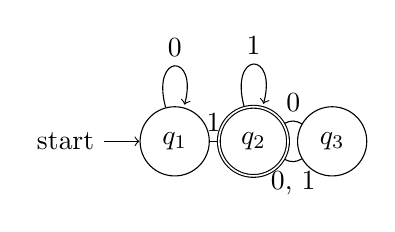
\begin{tikzpicture}
        \node[state, initial] (q1) {$q_1$};
        \node[state, accepting, right of=q1] (q2) {$q_2$};
        \node[state, right of=q2] (q3) {$q_3$};
        \draw (q1) edge[loop above] node{0} (q1)
        (q1) edge[above] node{1} (q2)
        (q2) edge[loop above] node{1} (q2)
        (q2) edge[bend left, above] node{0} (q3)
        (q3) edge[bend left, below] node{0, 1} (q2);
    \end{tikzpicture}

\end{document}